\documentclass{article}
\usepackage{graphicx}
\usepackage{listings}
\usepackage{ctex}
\usepackage{graphicx}
\usepackage[a4paper, body={18cm,22cm}]{geometry}
\usepackage{amsmath,amssymb,amstext,wasysym,enumerate,graphicx}
\usepackage{float,abstract,booktabs,indentfirst,amsmath}
\usepackage{array}
\usepackage{booktabs} %调整表格线与上下内容的间隔
\usepackage{multirow}
\usepackage{diagbox}
\usepackage{indentfirst}
\usepackage{bm}
\usepackage{fancyhdr}




\pagestyle{fancy}

\lhead{\bfseries \normalsize 学号:1952033\quad 姓名:侯雅玥 \quad 组员:廖宏 \\实验名称:集成运算放大电路的应用\quad 课程名称:电子技术实验\quad 专业:微电子科学与工程 } 
\rhead{}

\begin{document}
	\section{\zihao{4} 实验名称:集成运算放大电路的应用}
    \section{\zihao{4} 实验目的}
    \zihao {5} (1)通过对运算放大器几种基本电路的设计与测试,理解和认识放大器的工作原理及电路组成.\par
               (2)初步掌握集成运算放大器电路在实际应用中的设计方法和调试测量技术.\par
               (3)理解运算放大器的"虚地"、"虚短"、"虚断"等概念.
			   \section{\zihao{4} 实验原理}
			   集成运算放大器是具有高放大倍数的直接耦合放大电路,集成运算放大器必须工作在线性区.为了保证
			   运算放大器工作在线性区,电路中都引入了深度的负反馈.
               反相放大器和同相放大器是集成运算放大器的基本应用电路,许多集成运算放大器组成的功能电路都是
			   在反相和同相两种放大器的基础上组合演变而来的.
               理想集成运算放大器具有开环增益无限大、输入阻抗无限大、输出阻抗为零、带宽无限大、共模抑制比无限
			   大、失调及温漂为零等特性.实际运算放大器均能在一定程度上接近理想条件. 根据理想条件,由于运算放
			   大器引入深度负反馈,使集成运算放大器工作在线性范围,在应用时有两个重要特性∶\par
                (1)输出电压 $U_o$与输入电压之间满足关系式
				\begin{equation*}
					\ U_o=A_{ud}(U_+-U_-)
				\end{equation*}
              由于$A_{ud}=\infty$,而$U_o$为有限值,因此,$U_+-U_-\approx 0V$.即$U_+=U_-$,称为"虚短".\par
            (2)由于$R_i=\infty \Omega $,故流进运放两个输入端的电流可视为零,即$I_i=0A$,称为"虚断"\par
		反相比例放大电路
			反相比例放大电路,如图1所示.输入信号$U_i$,经电阻$R_l$,接到运算放大器的反相输入端,而同相输入端经
			过电阻$R_P$接地.输出电压$U_o$。经 $R_F$与 $R_l$,分压后反馈到反相输入端,构成一个闭环系统.反相比例放大器实际上是一个深度的电压并联负反馈电路.\par
			 由图1可知,在同相输入端,由于输入电流为零,$R_P$上没有压降,因此$U_o$=0V.又因在理想情况下,$U_-=U_+$,所以$U_-\approx 0V$,这种现象称为虚地."虚地"是反相放大器在闭环工作状态下的一个重要特点.\par
			由于从反相输入端流入集成运算放大器的电流为零,据此可以求得:
			\begin{equation*}
				\ A_{uF}=\frac{U_o}{U_i}=-\frac{R_F}{R_l}
			\end{equation*}
	           
		     \par
			即放大器的输出电压与输入电压的幅值成正比,但相位相反,比值$|A_{uF}|$取决于电阻$R_F$与$R_l$之比,而与集成运算放大器内部各参
			数无关.比值$|A_{uF}|$可以大于1,也可以小于1.当$R_i=R_l$时,$A_{uF}$=—1,这时电路称为单位增益倒相器或反相器.\par
			由于运算放大器的输入级均采用差分电路,因此在实际应用电路中,为了确保它的两个输入端处于平衡的工作状态,
			必须使输入级的偏流在两个输入端的外接电阻上产生相等的压降,以保持对称,避免产生附加的差动输入电压.为使反相输入
			端与同相输入端对地的电阻相等,直流平衡电阻 $R_P$应为$R_P=R_l||R_F$\par
			即放大器的输出电压与输入电压的幅值成正比,但相位相反,比值A。取决于电隙 R,与R,之比,而与集成运算放大器内部各参数无关. 
  
        电路输入阻抗为 $R_i\approx R_l$,这里,$R_F$不能取得太大,以免产生较大的噪声和漂移,其值一般取十至几百千欧,$R_l$应远大于信号源的内阻.\par
        同相比例放大电路、电压跟随器
         同相比例运算放大电路,如图2所示.输入信号 $U_i$,经电阻 $R_2$,接到运算放大器的同相输入端,反相输入端经 $R_l$,接地.为了保证电路稳定
		 工作,反馈信号仍需接到反相输入端.由图2可知,它是属于电压串联反馈.在同相比例运算放大器的实际电路中,也应使$R_2=R_l||R_F$,以保证
		 两个输入端对地的电阻相等.
        必须注意,同相比例运算放大电路的特点是∶集成运算放大器输入端存在着较高的共模输入电压,不存在虚地现象.又由于在图 2,$U_--U_+=U_i$,
		因此可以将两个输入端看成是虚拟短路.由此可以求出同相比例运算放大电路的电压放大倍数为
		\begin{equation*}
			\ A_{uF}=\frac{U_o}{U_i}=1+\frac{R_F}{R_l}
		\end{equation*}
		可以看出,$A_{uF}$总是大于或等于1.根据电压串联负反馈的特点,这种电路的输入电阻高,输出电阻低.\par
		在图2所示的电路中,当$R_f=0\Omega$(或 $R_l\infty\Omega$)时,由式$A_{uF}=\frac{U_o}{U_i}=1+\frac{R_F}{R_l}$可知$A_{uF}=1$,这时电路称为电压跟随器,如图3所示.此时输出电压
		与输入电压的关系为$U_o=U_i$,它与射极跟随器相似,具有良好的跟随和隔离作用.\par
		本实验可采用 LM358 集成电路
		
		\begin{figure}[h]
			\begin{minipage}[t]{0.33\linewidth} % 如果一行放2个图,用0.5,如果3个图,用0.33  
			  \centering   
			  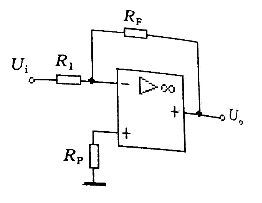
\includegraphics[width=2in]{H:/电子技术试验/4-12/4-12-12.png}   
			  \caption{反相放大器}   
			  \label{fig:side:a}   
			\end{minipage}%   
			\begin{minipage}[t]{0.33\linewidth}   
			  \centering   
			  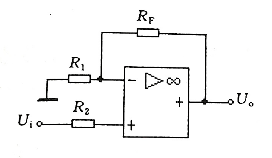
\includegraphics[width=2in]{H:/电子技术试验/4-12/4-12-13.png}   
			  \caption{同相放大器}   
			  \label{fig:side:b}   
			\end{minipage}   
			\begin{minipage}[t]{0.33\linewidth}   
				\centering   
				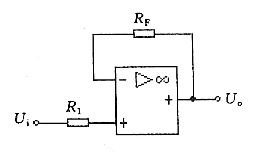
\includegraphics[width=2in]{H:/电子技术试验/4-12/4-12-14.png}   
				\caption{射极跟随器}   
				\label{fig:side:b}   
			  \end{minipage}  
		  \end{figure}
		 

\section{\zihao{4} 实验电路}

\begin{figure}[h]
	\begin{minipage}[t]{0.5\linewidth} % 如果一行放2个图,用0.5,如果3个图,用0.33  
	  \centering   
	  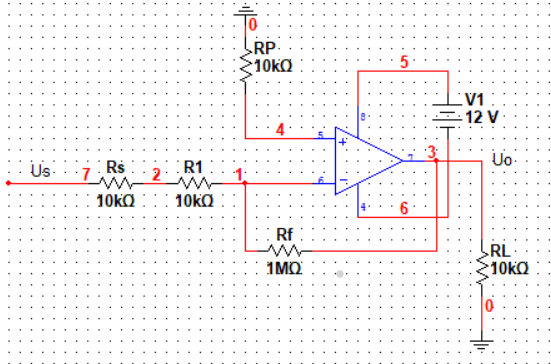
\includegraphics[width=3in]{H:/电子技术试验/4-12/4-12-6.png}   
	  \caption{反相放大器}   
	  \label{fig:side:a}   
	\end{minipage}%   
	\begin{minipage}[t]{0.5\linewidth}   
	  \centering   
	  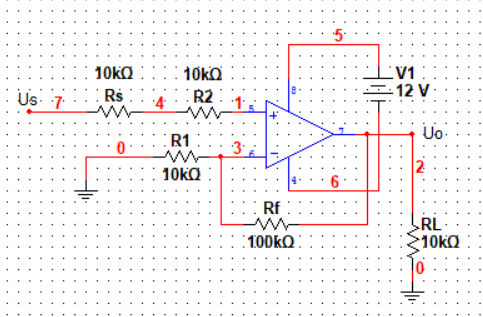
\includegraphics[width=3in]{H:/电子技术试验/4-12/4-12-7.png}   
	  \caption{同相放大器}   
	  \label{fig:side:b}   
	\end{minipage}   
  \end{figure}

\begin{figure}[h]
	%\small
	\centering
	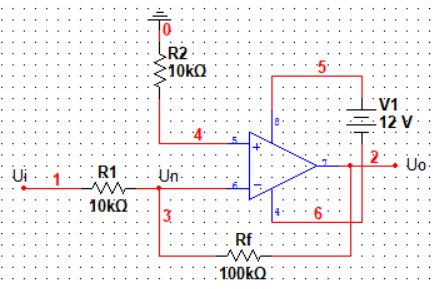
\includegraphics[width=3.6in]{H:/电子技术试验/4-12/4-12-8.png}
	\caption{反相放大器} \label{fig:aa}
\end{figure}

\section{\zihao{4} 实验内容及步骤}
\subsection {反相比例运算放大器的设计与调试}
(1)按照图4连接电路,断开$R_L$,即$R_L=+\infty$接通电源,调节输入正弦信号有效值$U_i$=30mV,f=1kHz,观察输入输出波形\par
(2)使$R_L=10k\Omega$接通电源,调节输入正弦信号有效值$U_i$=30mV,f=1kHz,观察输出波形
\subsection{同相比例运算放大器的设计与调试}
(1)按照图5连接电路,断开$R_L$,即$R_L=+\infty$接通电源,调节输入正弦信号有效值$U_i$=80mV,f=1kHz,观察输入输出波形\par
(2)使$R_L=10k\Omega$$U_i$=80mV,f=1kHz,观察输出波形
\subsection{反相比例运算放大器}
(1)按照图6连接电路,接通电源,调节输入三角波信号峰峰值值$U_{p-p}$=1V,f=1kHz,观察$U_o,U_n$输出波形\par
(1)调节输入三角波信号峰峰值值$U_{p-p}$=3V,f=1kHz,观察$U_o,U_n$输出波形\par
\newpage	
\section{\zihao{4} 数据处理}
	\subsection {反相比例运算放大器的设计与调试}
	
	\begin{figure}[h]
		\begin{minipage}[t]{0.5\linewidth} % 如果一行放2个图,用0.5,如果3个图,用0.33  
		  \centering   
		  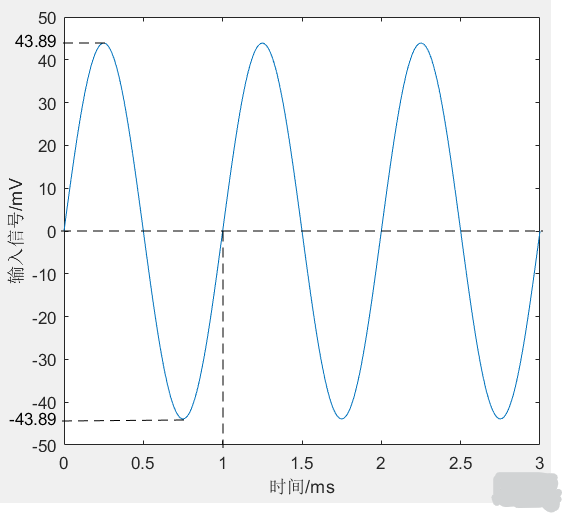
\includegraphics[width=2.6in]{H:/电子技术试验/4-12/4-12-1.png}   
		  \caption{输入信号}   
		  \label{fig:side:a}   
		\end{minipage}%   
		\begin{minipage}[t]{0.5\linewidth}   
		  \centering   
		  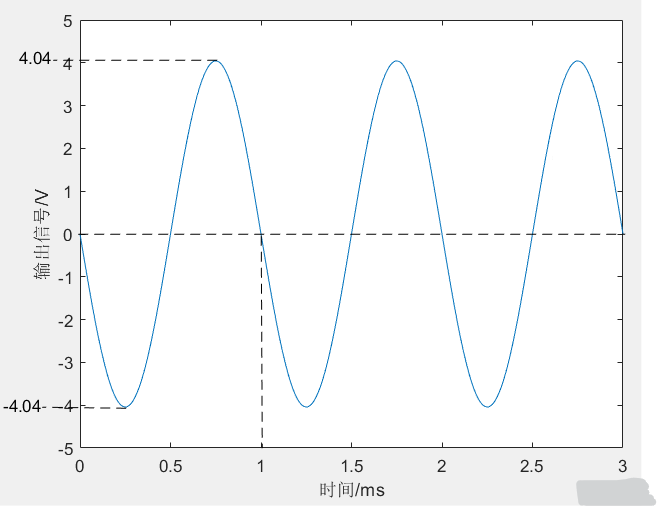
\includegraphics[width=3in]{H:/电子技术试验/4-12/4-12-2.png}   
		  \caption{$R_L=\infty$时输出信号}   
		  \label{fig:side:b}   
		\end{minipage}   
		
	  \end{figure}
	
	\begin{figure}[h]
		%\small
		\centering
		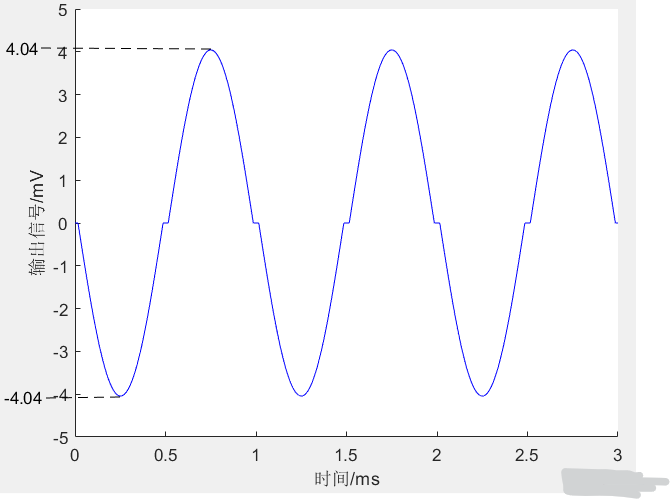
\includegraphics[width=3in]{H:/电子技术试验/4-12/4-12-3.png}
		\caption{$R_L=10k\Omega$时的输出波形} \label{fig:aa}
	\end{figure}
	\par
计算得
\begin{equation*}
	\ A_{uF}=\frac{U_o}{U_i}=92
\end{equation*}\par
理论值
\begin{equation*}
	\ A_{uF0}=\frac{U_o}{U_i}=-\frac{R_F}{R_L}=100
\end{equation*}\par
相对误差
\begin{equation*}
	\ \delta_{A_{uF}}=\frac{A_{uF0}-A_{uF}}{A_{uF}}=8.6\%
\end{equation*}
	\newpage
	\subsection {同相比例运算放大器的设计与调试}
	\begin{figure}[h]
		\begin{minipage}[t]{0.5\linewidth} % 如果一行放2个图,用0.5,如果3个图,用0.33  
		  \centering   
		  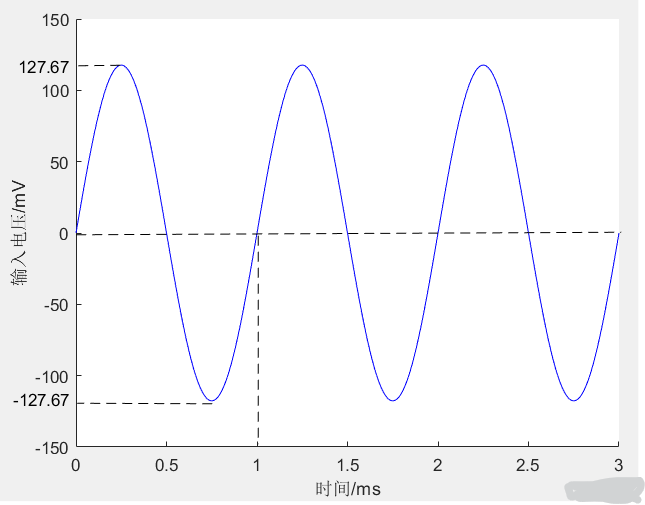
\includegraphics[width=3.5in]{H:/电子技术试验/4-12/4-12-4.png}   
		  \caption{输入信号}   
		  \label{fig:side:a}   
		\end{minipage}%   
		\begin{minipage}[t]{0.5\linewidth}   
		  \centering   
		  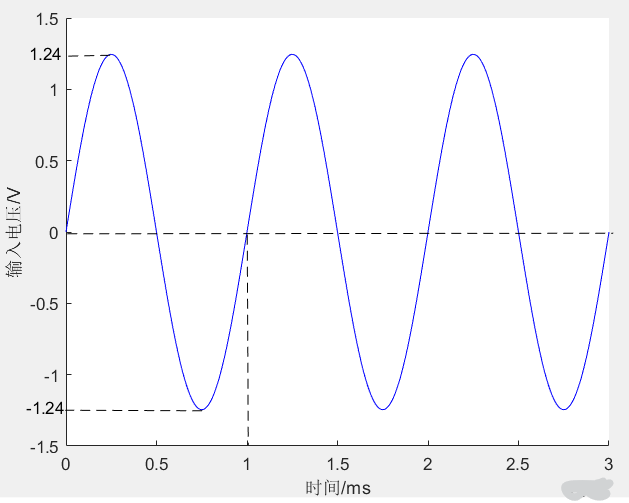
\includegraphics[width=3.5in]{H:/电子技术试验/4-12/4-12-11.png}   
		  \caption{$R_L=\infty$时输出信号}   
		  \label{fig:side:b}   
		\end{minipage}   
		
	  \end{figure}
   
	\begin{figure}[h]
		%\small
		\centering
		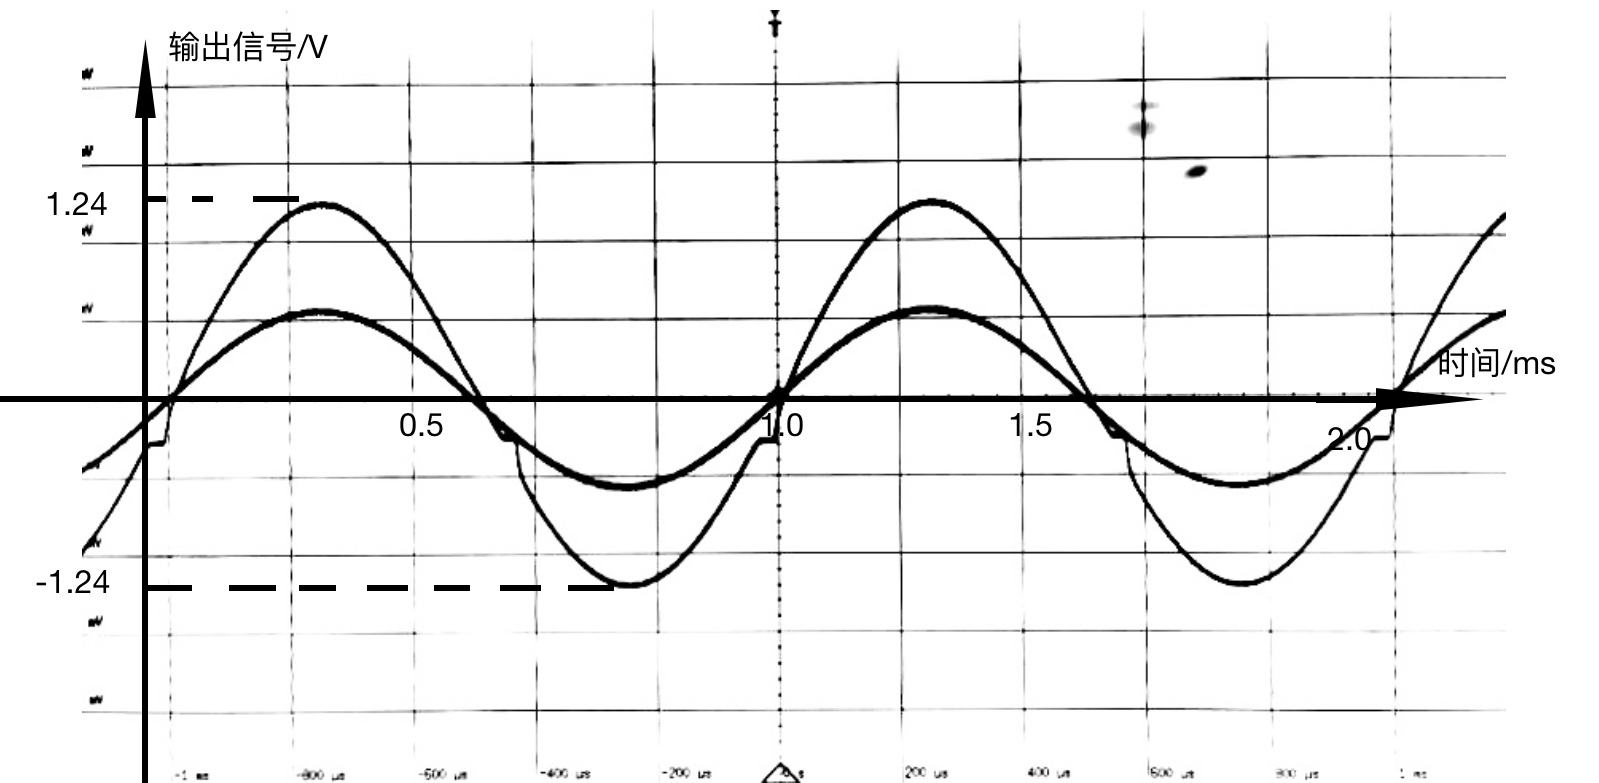
\includegraphics[width=12cm]{H:/电子技术试验/4-12/4-12-5.png}
		\caption{$R_L=10k\Omega$时的输出波形} \label{fig:aa}
	\end{figure}
	计算得
	\begin{equation*}
		\ A_{uF}=\frac{U_o}{U_i}=10
	\end{equation*}\par
	理论值
	\begin{equation*}
		\ A_{uF0}=\frac{U_o}{U_i}=1+\frac{R_F}{R_L}=11
	\end{equation*}\par
	相对误差
	\begin{equation*}
		\ \delta_{A_{uF}}=\frac{A_{uF0}-A_{uF}}{A_{uF}}=10\%
	\end{equation*}
		\newpage
	\par
	\subsection {反相比例运算放大器的虚短}
	输入输出波形$U_{p-p}=1V$:
	\begin{figure}[h]
		%\small
		\centering
		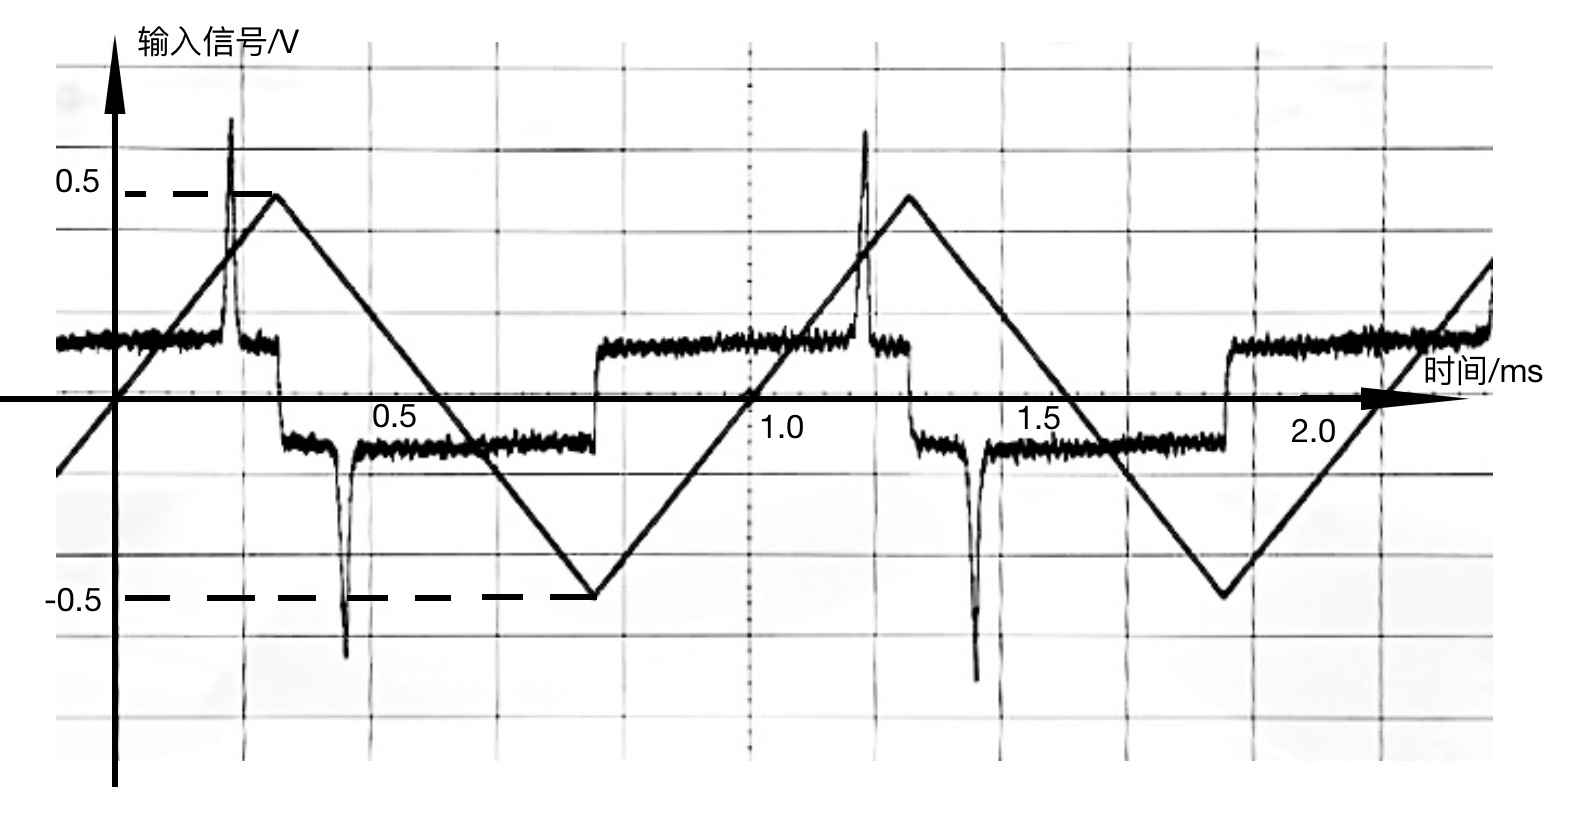
\includegraphics[width=10cm]{H:/电子技术试验/4-12/4-12-9.png}
		\caption{$U_{p-p}=1V$} \label{fig:aa}
	\end{figure}
\par
	输入输出波形$U_{p-p}=3V$:
	\begin{figure}[h]
		%\small
		\centering
		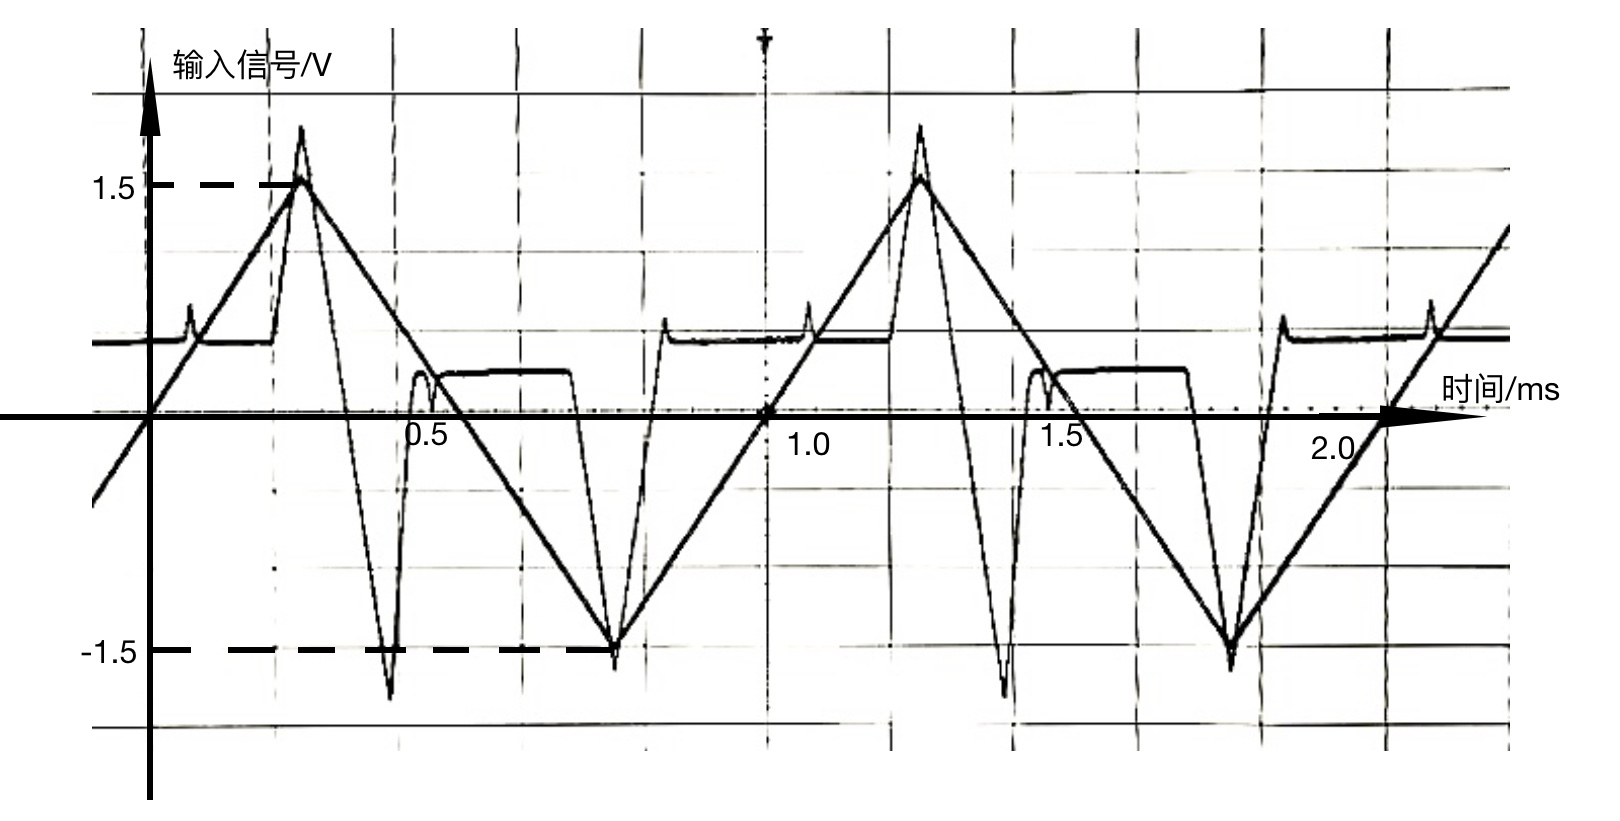
\includegraphics[width=10cm]{H:/电子技术试验/4-12/4-12-10.png}
		\caption{$U_{p-p}=3V$} \label{fig:aa}
	\end{figure}

	\section{\zihao{4} 实验设备和器材}
	(1)双踪示波器             \qquad \qquad \qquad \qquad \qquad  \qquad           1台\par
	(2)函数信号发生器          \qquad  \qquad \qquad \qquad       \qquad           1台\par
	(3)直流稳压电源             \qquad \quad \qquad \qquad \qquad \qquad           1台\par
	(4)模拟电路实验箱            \qquad  \qquad \qquad \qquad\qquad                1台\par
	(5)万用表                   \qquad  \qquad \qquad \qquad \qquad \qquad \qquad  1只\par
	(6)集成芯片LM358、电阻器、电容器  \quad                                        若干

\section{结论}
(1)反相放大器的输入电阻$R_i=\infty$,输入端之间虚断,且$ A_{uF0}=\frac{U_o}{U_i}=-\frac{R_F}{R_L}$\par
(1)同相放大器$ A_{uF0}=\frac{U_o}{U_i}=1+\frac{R_F}{R_L}$

\section{思考题}
(1)在理想运算放大器情况下,从反相放大器信号源两端向放大器看进去,输入电阻为多少? 它有何特点?\par
这时的输入电阻趋近无穷大,因为两输入端之间虚断.\par
(2)理想的运算放大器具有哪些特点?\par
输入阻抗无限大$R_i=\infty$;输出阻抗趋近于零$R_o=0$;开回路增益无限大$A_{uF}=\infty$;共模抑制比无限大$CMRR=\infty$;带宽无限大.\par
(3)电压跟随器在多级放大器中的位置应如何确定?\par
电压跟随器一般用于多级放大电路的输入级、输出级,也可连接两电路,起缓冲作用。
由于电压跟随器输入电阻大,输出电阻小,因此也可以用来做阻抗转换,增大放大器后级的带负载能力。一般做射极跟随器。 \par
(4)为了不损坏集成块,实验中应注意什么问题?\par
实验前要看清运放器件各管脚的位置;切忌正、负电源极性接反和输出端短路,以免损坏集成块.

\end{document}

